% =====================================================================
%  Back cover — Dark Matter
%  Typeset standalone at the 6 x 9 in trim, full bleed.
%  Vertical positions are measured in inches from the foot of the page.
% =====================================================================
\documentclass{article}
\usepackage[paperwidth=6in,paperheight=9in,margin=0pt]{geometry}
\usepackage{fontspec}
\usepackage{xcolor}
\usepackage{graphicx}
\usepackage{tikz}

\setmainfont{Outfit}[
  UprightFont={Outfit Regular}, BoldFont={Outfit Bold},
  ItalicFont={Outfit Regular}, ItalicFeatures={FakeSlant=0.20},
  BoldItalicFont={Outfit Bold}, BoldItalicFeatures={FakeSlant=0.20},
  Ligatures={TeX}]
\setsansfont{Outfit}[
  UprightFont={Outfit Regular}, BoldFont={Outfit Bold},
  ItalicFont={Outfit Regular}, ItalicFeatures={FakeSlant=0.20},
  BoldItalicFont={Outfit Bold}, BoldItalicFeatures={FakeSlant=0.20},
  Ligatures={TeX}]
\setmonofont{DejaVu Sans Mono}[
  UprightFont={DejaVu Sans Mono}, BoldFont={DejaVu Sans Mono Bold},
  Ligatures={TeX}]

\definecolor{ink}{HTML}{0B0E1A}
\definecolor{accent}{HTML}{F0C36A}
\definecolor{txt}{HTML}{E8EAF0}
\definecolor{dim}{HTML}{98A0B0}

\pagestyle{empty}
\setlength{\parindent}{0pt}

\begin{document}
\begin{tikzpicture}[remember picture,overlay]
  % ---- the plate, full bleed (a different crop from the front) ----------
  \node[anchor=south west,inner sep=0] at (current page.south west)
    {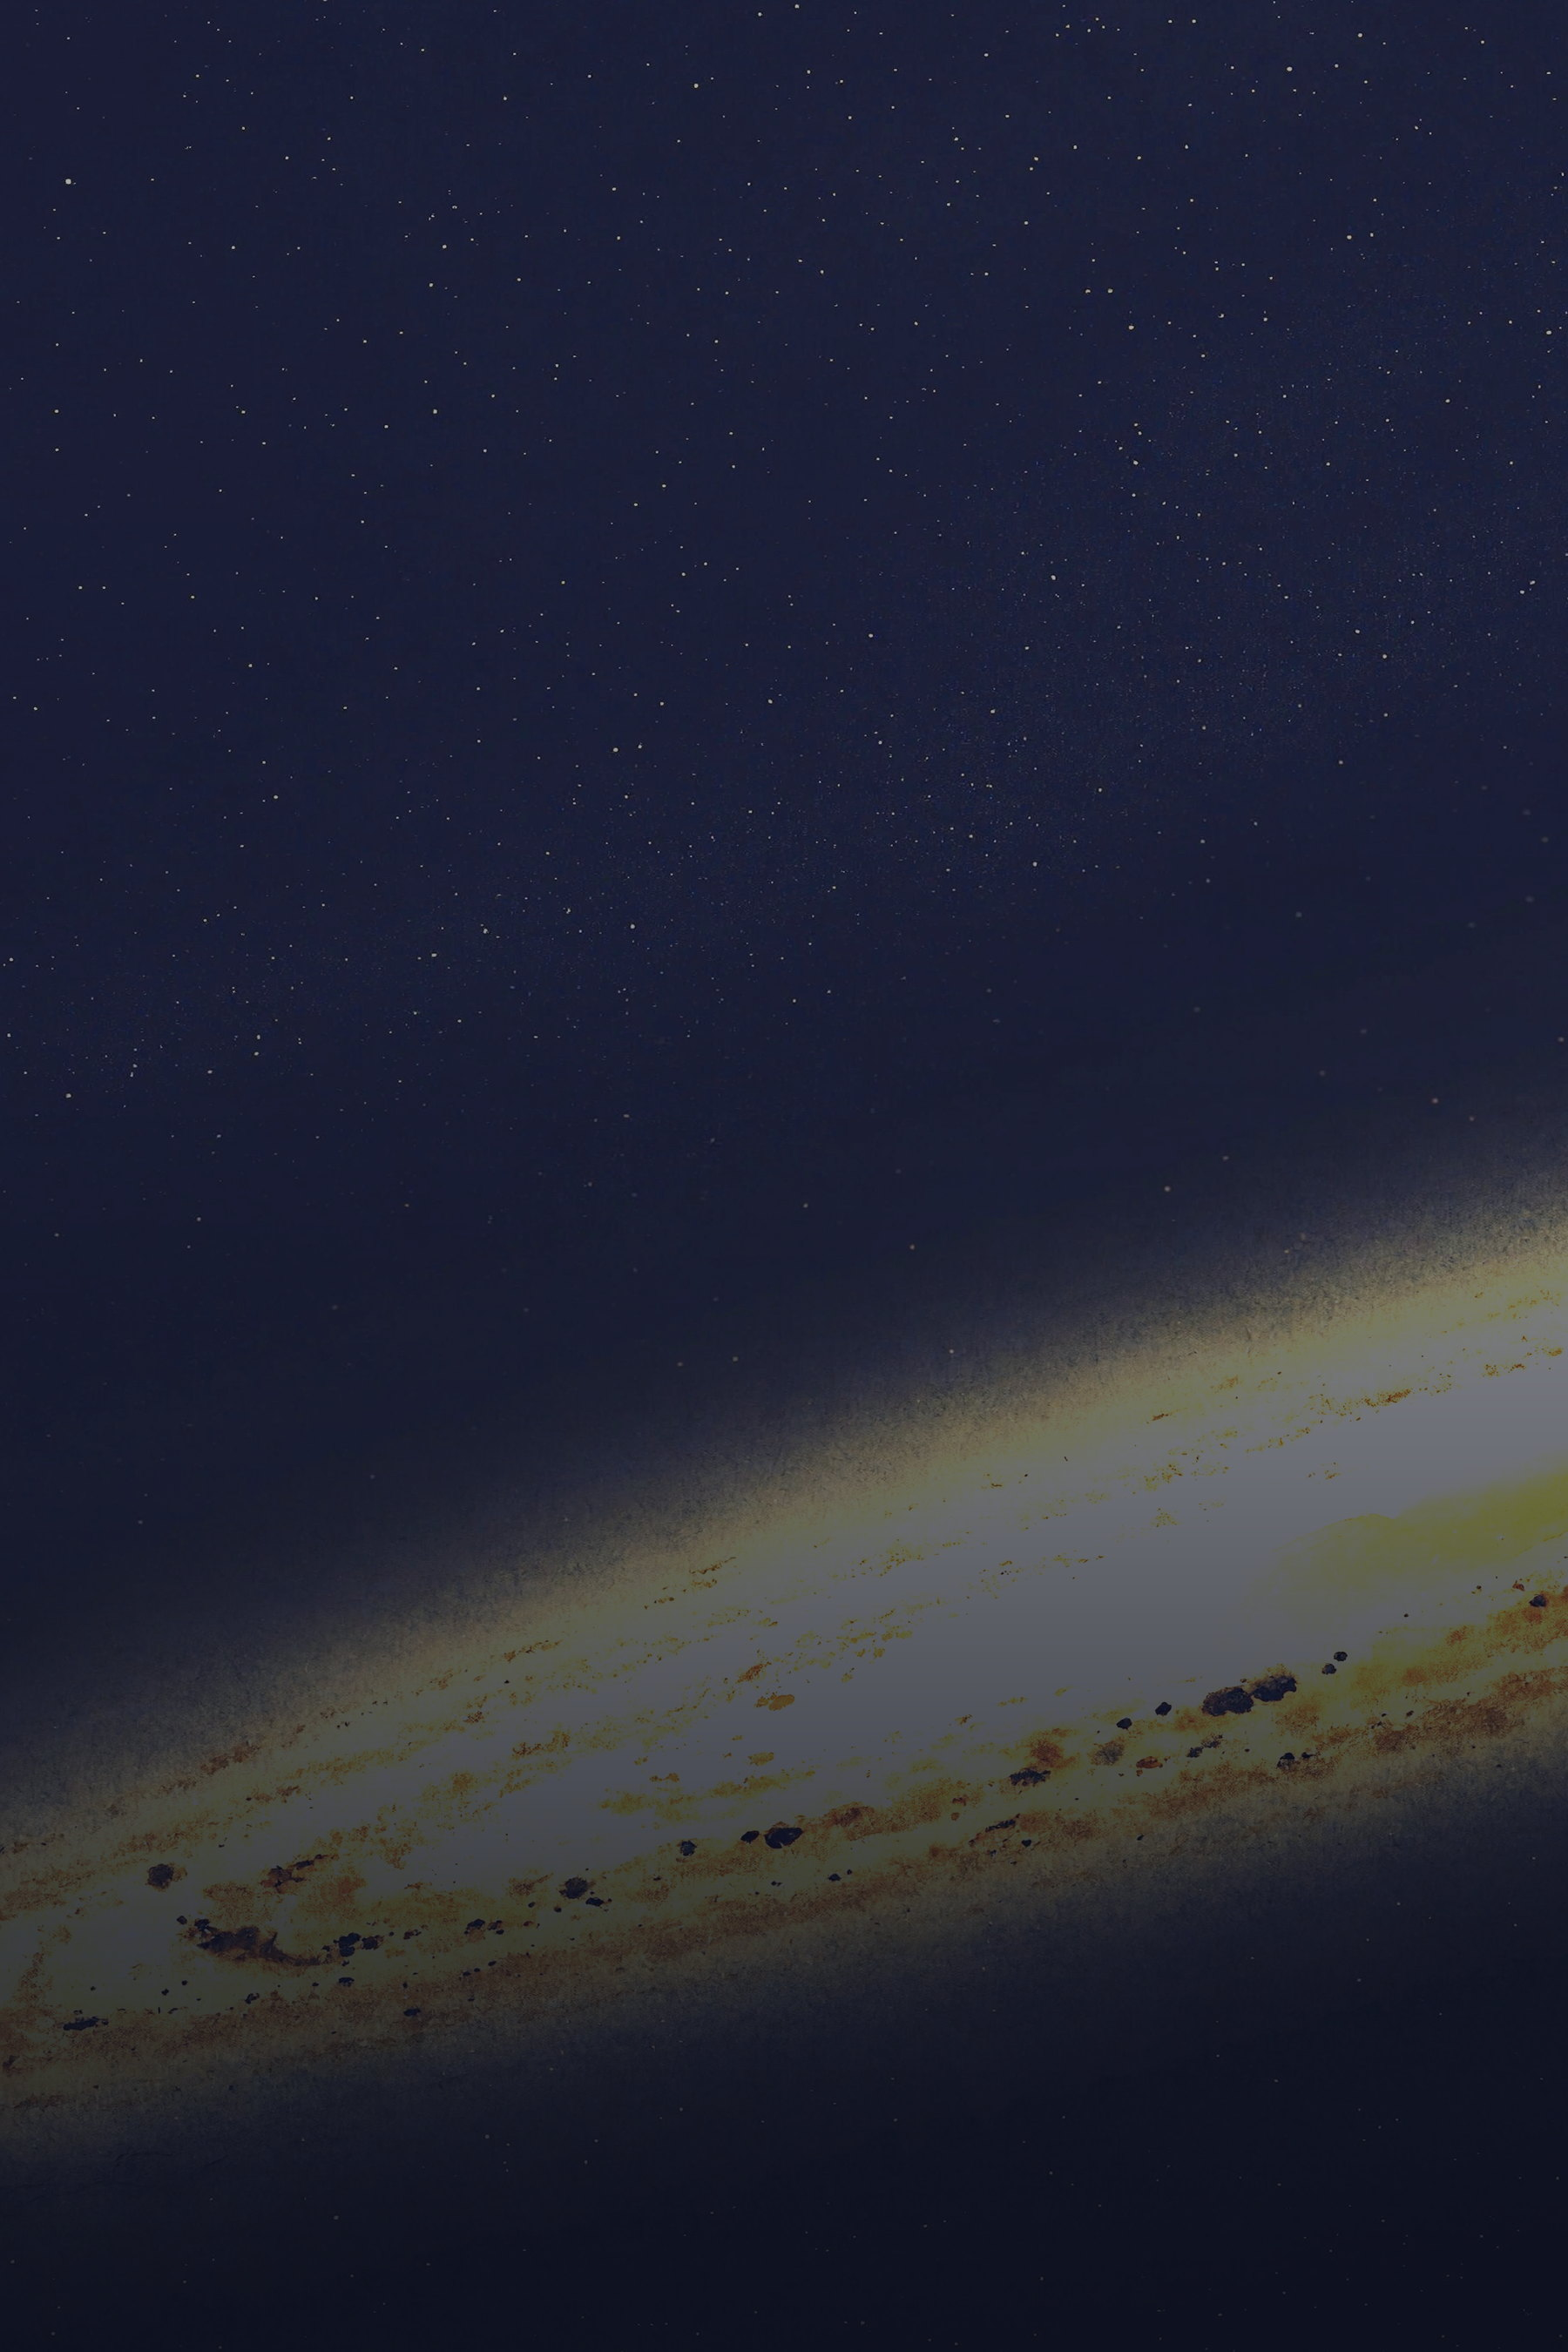
\includegraphics[width=\paperwidth,height=\paperheight]{../figures/cover_back_art.jpg}};

  % ---- title strip -------------------------------------------------------
  \node[anchor=south west,inner sep=0,text=accent] at ([xshift=0.60in,yshift=8.26in]current page.south west)
    {\fontsize{9.2}{11}\selectfont\sffamily\bfseries
     {\addfontfeatures{LetterSpace=15}DARK MATTER}};

  \fill[accent] ([xshift=0.60in,yshift=8.00in]current page.south west)
         rectangle ([xshift=5.48in,yshift=8.02in]current page.south west);

  \node[anchor=south west,inner sep=0,text=dim] at ([xshift=0.60in,yshift=7.66in]current page.south west)
    {\fontsize{9.8}{12}\selectfont\sffamily Gerald Enrique Nelson Mc Kenzie};

  % ---- blurb -------------------------------------------------------------
  \node[anchor=north west,inner sep=0,text=txt,align=left] at ([xshift=0.60in,yshift=7.24in]current page.south west)
    {\fontsize{8.1}{11.0}\selectfont\sffamily
     Dark matter is 26.8 per cent of the universe's energy density and 84 per\\
     cent of its matter. The density is known to two per cent. The particle\\
     is not known at all.\\[7pt]
     This book is an assessment of the field as it stands in late 2026: what\\
     the evidence establishes, which candidates remain viable and on what\\
     grounds, and what should be built, funded and decided next.\\[7pt]
     It takes the live 248 keV candidate seriously and applies to it the\\
     standard the field wrote down. It audits the anomaly record of the last\\
     five years, four of which did not replicate.\\[7pt]
     And it answers the question the title asks, in five senses. We have used\\
     dark matter as a gravitational probe for ninety years, and captured a\\
     private supply of it in the Solar System, where the local density is\\
     enhanced by orders of magnitude. We have, on paper, harvested it.\\[7pt]
     The interesting senses have positive answers. The particle sense does\\
     not. The distance between those two facts is the distance the field has\\
     to close.};

  % ---- parts -------------------------------------------------------------
  \node[anchor=south west,inner sep=0,text=accent] at ([xshift=0.60in,yshift=3.62in]current page.south west)
    {\fontsize{6.8}{8}\selectfont\sffamily\bfseries {\addfontfeatures{LetterSpace=18}INSIDE}};

  \node[anchor=north west,inner sep=0,text=txt,align=left] at ([xshift=0.60in,yshift=3.48in]current page.south west)
    {\fontsize{8.4}{11.4}\selectfont\sffamily
     I \quad The Budget and the Evidence\\
     II \quad The Candidate Landscape\\
     III \quad The Frontier\\
     IV \quad The Origins\\
     V \quad Have We Already Tapped It?\\
     VI \quad The Decision};

  % ---- footer ------------------------------------------------------------
  \fill[dim,opacity=0.45] ([xshift=0.60in,yshift=0.92in]current page.south west)
         rectangle ([xshift=5.48in,yshift=0.93in]current page.south west);

  \node[anchor=south west,inner sep=0,text=dim] at ([xshift=0.60in,yshift=0.66in]current page.south west)
    {\fontsize{7.6}{9.6}\selectfont\sffamily
     Tico Internet LLC \quad\textperiodcentered\quad 2026 First Edition
     \quad\textperiodcentered\quad Apache License 2.0};

  \node[anchor=south west,inner sep=0,text=dim] at ([xshift=0.60in,yshift=0.46in]current page.south west)
    {\fontsize{7.6}{9.6}\selectfont\sffamily DOI 10.5281/zenodo.24435288};
\end{tikzpicture}
\null
\end{document}
